\documentclass[tikz,border=10pt]{standalone}
\begin{document}
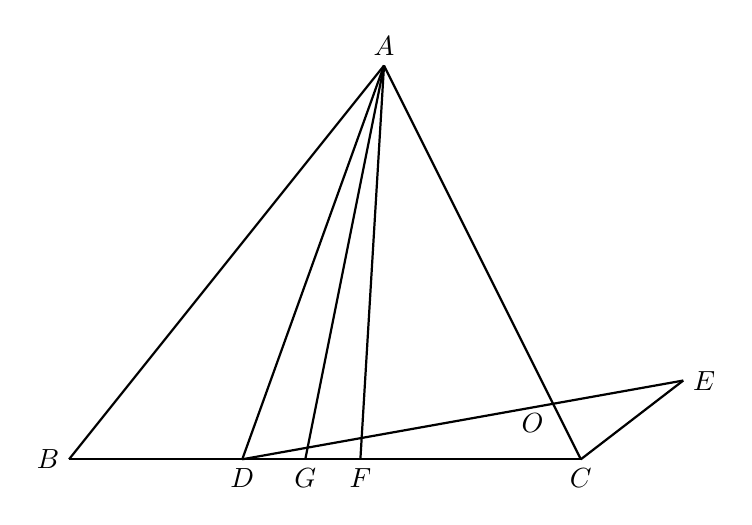
\begin{tikzpicture}[scale=1]
\coordinate (A) at (0,5);
\coordinate (B) at (-4,0);
\coordinate (C) at (2.5,0);
\coordinate (D) at (-1.8,0);
\coordinate (G) at (-1,0);
\coordinate (F) at (-0.3,0);
\coordinate (O) at (2.15,0.7);
\coordinate (E) at (3.8,1);

\draw[thick] (B) -- (C);
\draw[thick] (A) -- (B);
\draw[thick] (A) -- (C);
\draw[thick] (A) -- (D);
\draw[thick] (A) -- (G);
\draw[thick] (A) -- (F);
\draw[thick] (D) -- (E);
\draw[thick] (C) -- (E);

\node[above] at (A) {$A$};
\node[left] at (B) {$B$};
\node[below] at (C) {$C$};
\node[below] at (D) {$D$};
\node[below] at (G) {$G$};
\node[below] at (F) {$F$};
\node[below left] at (O) {$O$};
\node[right] at (E) {$E$};
\end{tikzpicture}
\end{document}
